\chapter{Estudio de requisitos}

\section{Actores}

El producto final de este proyecto es un port que en el futuro un desarrollador utilizará para crear un proyecto. Por tanto, en el análisis de requisitos, este futuro desarrollador es el principal y único actor. \autoref{AC-01}.

\begin{table}[!ht]
    \begin{tabular}{|llllll|}
	\hline
	\multicolumn{1}{|l|}{\textbf{Actor}}		& \multicolumn{4}{l|}{Desarrollador}	& AC-01	    \\ \hline
	\multicolumn{1}{|l|}{\textbf{Descripción}}     	& \multicolumn{5}{l|}{Persona que utiliza el port para hacer un proyecto con la placa}	    \\ \hline
	% \multicolumn{1}{|l|}{\textbf{Características}}	& \multicolumn{5}{l|}{Programar}	\\ \hline
	% \multicolumn{1}{|l|}{\textbf{Relaciones}}		& \multicolumn{5}{l|}{Diseña tareas que luego FreeRTOS ejecuta}	    \\ \hline
	\multicolumn{1}{|l|}{\textbf{Referencias}}     	& \multicolumn{5}{l|}{RF0, RF1}	\\ \hline
	\multicolumn{1}{|l|}{\textbf{Autor}}           	& \multicolumn{1}{l|}{Enrique Paubert}        & \multicolumn{1}{l|}{\textbf{Fecha}}        & \multicolumn{1}{l|}{10/08/2024}        & \multicolumn{1}{l|}{\textbf{Versión}}       & 1.0                   \\ \hline
	% \multicolumn{6}{|l|}{\textbf{\underline{Atributos}}} \\ \hline % \cellcolor[HTML]{DAE8FC}
	% \multicolumn{1}{|l|}{\textbf{Nombre}}		& \multicolumn{4}{l|}{\textbf{Descripción}} &  \textbf{Tipo}  \\ \hline
	% \multicolumn{1}{|l|}{ - }				& \multicolumn{4}{l|}{ - }  &  -      \\ \hline
    \end{tabular}
    \caption[Actor: Desarrollador]{Especificación del actor Desarrollador.}
    \label{AC-01}
\end{table}

\section{Casos de Uso}

Los casos de uso recogerán las interacciones que puede tener el futuro desarrollador con el port. Tablas \ref{CU-01}, \ref{CU-02}, \ref{CU-03} y \ref{CU-04}.

\begin{table}[!ht]
    \begin{tabular}{|l|l|l|l|l|l|}
	\hline
	\textbf{Caso de Uso} & \multicolumn{3}{l|}{Configurar el sistema} & \multicolumn{2}{l|}{CU-01} \\ \hline
	\textbf{Actores} & \multicolumn{5}{l|}{Desarrollador} \\ \hline
	\textbf{Tipo} & \multicolumn{5}{l|}{Primario, Esencial} \\ \hline
	\textbf{Referencias} & RF0 & \multicolumn{4}{l|}{-} \\ \hline
	\textbf{Precondición} & \multicolumn{5}{l|}{El sistema tiene una configuración concreta} \\ \hline
	\textbf{Postcondición} & \multicolumn{5}{l|}{La configuración del sistema ha cambiado} \\ \hline
	\textbf{Autor} & Enrique Paubert & \textbf{Fecha} & 10/08/2024 & \textbf{Versión} & 1.0 \\ \hline
	% \multicolumn{6}{|l|}{\textbf{\underline{Propósito}}} \\ \hline %\cellcolor[HTML]{ECF4FF}
	% \multicolumn{6}{|l|}{Que el desarrollador pueda configurar el sistema según sus necesidades} \\ \hline
	% \multicolumn{6}{|l|}{\textbf{\underline{Resumen}}} \\ \hline % \cellcolor[HTML]{ECF4FF}
	% \multicolumn{6}{|l|}{\begin{tabular}[c]{@{}l@{}}1. El desarollador configura el sistema.\\  2. -. \\ 3. profit.\end{tabular}} \\ \hline
    \end{tabular}%
    \caption{Caso de uso de configurar el sistema}
    \label{CU-01}
\end{table}

\begin{table}[!ht]
    \begin{tabular}{|l|l|l|l|l|l|}
	\hline
	\textbf{Caso de Uso} & \multicolumn{3}{l|}{Diseñar una tarea} & \multicolumn{2}{l|}{CU-02} \\ \hline
	\textbf{Actores} & \multicolumn{5}{l|}{Desarrollador} \\ \hline
	\textbf{Tipo} & \multicolumn{5}{l|}{Primario, Esencial} \\ \hline
	\textbf{Referencias} & RF1 & \multicolumn{4}{l|}{-} \\ \hline
	\textbf{Precondición} & \multicolumn{5}{l|}{-} \\ \hline
	\textbf{Postcondición} & \multicolumn{5}{l|}{Existe una función que puede actuar como tarea} \\ \hline
	\textbf{Autor} & Enrique Paubert & \textbf{Fecha} & 10/08/2024 & \textbf{Versión} & 1.0 \\ \hline
	% \multicolumn{6}{|l|}{\textbf{\underline{Propósito}}} \\ \hline %\cellcolor[HTML]{ECF4FF}
	% \multicolumn{6}{|l|}{El desarrollador diseña una tarea} \\ \hline
	% \multicolumn{6}{|l|}{\textbf{\underline{Resumen}}} \\ \hline % \cellcolor[HTML]{ECF4FF}
	% \multicolumn{6}{|l|}{\begin{tabular}[c]{@{}l@{}}1. El desarollador crea una tarea.\\  2. -. \\ 3. profit.\end{tabular}} \\ \hline
    \end{tabular}%
    \caption{Caso de uso de diseñar una tarea}
    \label{CU-02}
\end{table}

\begin{table}[!ht]
    \begin{tabular}{|l|l|l|l|l|l|}
	\hline
	\textbf{Caso de Uso} & \multicolumn{3}{l|}{Crear una instancia de una tarea} & \multicolumn{2}{l|}{CU-03} \\ \hline
	\textbf{Actores} & \multicolumn{5}{l|}{Desarrollador} \\ \hline
	\textbf{Tipo} & \multicolumn{5}{l|}{Primario, Esencial} \\ \hline
	\textbf{Referencias} & RF1 & \multicolumn{4}{l|}{-} \\ \hline
	\textbf{Precondición} & \multicolumn{5}{l|}{Existe una función que puede actuar como tarea} \\ \hline
	\textbf{Postcondición} & \multicolumn{5}{l|}{Se añadirá una instancia de esta tarea al sistema} \\ \hline
	\textbf{Autor} & Enrique Paubert & \textbf{Fecha} & 10/08/2024 & \textbf{Versión} & 1.0 \\ \hline
	% \multicolumn{6}{|l|}{\textbf{\underline{Propósito}}} \\ \hline %\cellcolor[HTML]{ECF4FF}
	% \multicolumn{6}{|l|}{???} \\ \hline
	% \multicolumn{6}{|l|}{\textbf{\underline{Resumen}}} \\ \hline % \cellcolor[HTML]{ECF4FF}
	% \multicolumn{6}{|l|}{\begin{tabular}[c]{@{}l@{}}1. El desarollador crea una tarea.\\  2. -. \\ 3. profit.\end{tabular}} \\ \hline
    \end{tabular}%
    \caption{Caso de uso de crear una instancia de una tarea}
    \label{CU-03}
\end{table}

\begin{table}[!ht]
    \begin{tabular}{|l|l|l|l|l|l|}
	\hline
	\textbf{Caso de Uso} & \multicolumn{3}{l|}{Eliminar una instancia de una tarea} & \multicolumn{2}{l|}{CU-04} \\ \hline
	\textbf{Actores} & \multicolumn{5}{l|}{Desarrollador} \\ \hline
	\textbf{Tipo} & \multicolumn{5}{l|}{Primario, Esencial} \\ \hline
	\textbf{Referencias} & RF1 & \multicolumn{4}{l|}{-} \\ \hline
	\textbf{Precondición} & \multicolumn{5}{l|}{Hay una instancia de una tarea en el sistema} \\ \hline
	\textbf{Postcondición} & \multicolumn{5}{l|}{Se elimina dicha instancia de la tarea del sistema} \\ \hline
	\textbf{Autor} & Enrique Paubert & \textbf{Fecha} & 10/08/2024 & \textbf{Versión} & 1.0 \\ \hline
	% \multicolumn{6}{|l|}{\textbf{\underline{Propósito}}} \\ \hline %\cellcolor[HTML]{ECF4FF}
	% \multicolumn{6}{|l|}{???} \\ \hline
	% \multicolumn{6}{|l|}{\textbf{\underline{Resumen}}} \\ \hline % \cellcolor[HTML]{ECF4FF}
	% \multicolumn{6}{|l|}{\begin{tabular}[c]{@{}l@{}}1. El desarollador crea una tarea.\\  2. -. \\ 3. profit.\end{tabular}} \\ \hline
    \end{tabular}%
    \caption{Caso de uso de eliminar una instancia de una tarea}
    \label{CU-04}
\end{table}

\section{Diagramas de casos de uso}
En este diagrama mostraré cómo el desarrollador interacciona con el sistema. \autoref{fig:UML}.

\begin{figure}[!ht]
\centering
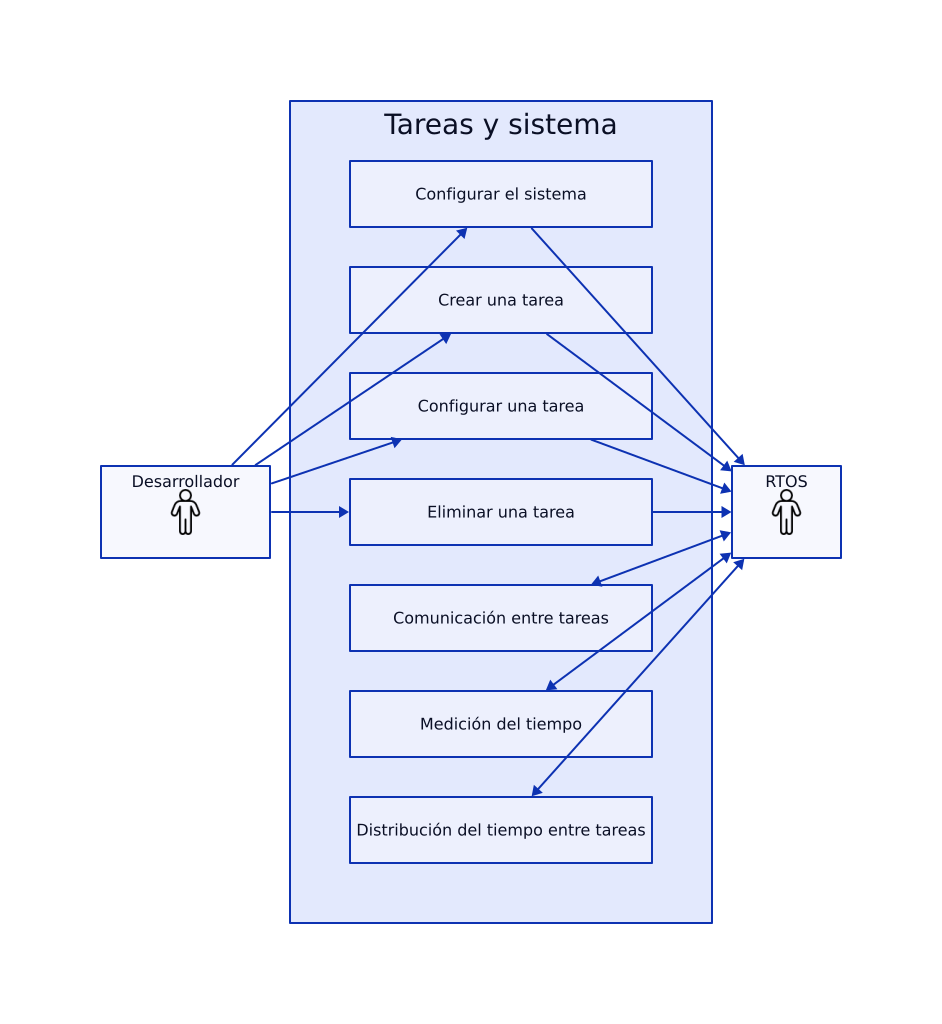
\includegraphics[width=\textwidth]{img/UML1.png}
\caption{Diagrama UML de las tareas}
\label{fig:UML}
\end{figure}

\section{Requisitos}
Los requisitos funcionales describen especifican qué debe de hacer el sistema, mientras que los no funcionales describen cómo debe de hacerlo.

\subsection{Requisitos no funcionales}
Empezaremos listando los requisitos no funcionales ya que imponen ciertas restricciones esenciales que afectan al diseño del sistema.

% \subsubsection{Uso obligatorio de FreeRTOS:}
% El sistema debe usar FreeRTOS como el sistema operativo en tiempo real (RTOS). Este proyecto fue concebido en un principio para utilizar FreeRTOS.
%
% \subsubsection{Uso obligatorio de la Redwire Econotag R3:}
% El port debe estar diseñado para funcionar en la placa Redwire Econotag R3. Esta placa es la utilizada en la asignatura de sistema empotrados. Dado que este proyecto se plantea como una profundización en esta asignatura, tiene sentido utilizar la misma placa.
%
% \subsubsection{Uso del BSP desarrollado en SE:}
% Se debe utilizar un BSP desarrollado en una asignatura de sistemas empotrados. Al igual que en el requisito anterior, se debe a que este proyecto es una expansión de esa asignatura.
%
% \subsubsection{Eficiencia del sistema:}
% El sistema debe ser eficiente en cuanto a consumo de recursos, minimizando el uso de CPU y memoria. Dado que se trata de un sistema embebido con recursos limitados, es crucial optimizar el uso de los mismos.
%
% \subsubsection{Documentación y mantenibilidad:}
% El código y la configuración del sistema deben estar bien documentados para facilitar su mantenimiento y posibles futuras modificaciones. La calidad de la documentación es crucial para el mantenimiento a largo plazo y para la colaboración con otros desarrolladores.
%

\begin{itemize}
    \item \textbf{RNF-01 - Uso obligatorio de FreeRTOS:} El sistema debe usar FreeRTOS como el sistema operativo en tiempo real (RTOS). Este proyecto fue concebido en un principio para utilizar FreeRTOS.
    \item \textbf{RNF-02 - Uso obligatorio de la Redwire Econotag R3:} El port debe estar diseñado para funcionar en la placa Redwire Econotag R3. Esta placa es la utilizada en la asignatura de sistema empotrados. Dado que este proyecto se plantea como una profundización en esta asignatura, tiene sentido utilizar la misma placa.
    \item \textbf{RNF-03 - Uso del BSP desarrollado en SE:} Se debe utilizar un BSP desarrollado en una asignatura de sistemas empotrados. Al igual que en el requisito anterior, se debe a que este proyecto es una expansión de esa asignatura.
    \item \textbf{RNF-04 - Eficiencia del sistema:} El sistema debe ser eficiente en cuanto a consumo de recursos, minimizando el uso de CPU y memoria. Dado que se trata de un sistema embebido con recursos limitados, es crucial optimizar el uso de los mismos.
    \item \textbf{RNF-05 - Documentación y mantenibilidad:} El código y la configuración del sistema deben estar bien documentados para facilitar su mantenimiento y posibles futuras modificaciones. La calidad de la documentación es crucial para el mantenimiento a largo plazo y para la colaboración con otros desarrolladores.
\end{itemize}

\subsection{Requisitos funcionales}

% \subsubsection{Tiempo real}
% El port debe de garantizar que el sistema funcione con restricciones de tiempo real.
%
% \subsubsection{Gestión de tareas:}
% El sistema debe permitir la correcta creación, gestión y eliminación de tareas.
%
% \subsubsection{Soporte para periféricos:}
% El port debe incluir, mediante el BSP, soporte para los periféricos principales de la Econotag, (GPIO, UART...).
%
% \subsubsection{Configuración del Sistema}
% El sistema debe permitir la configuración de parámetros de FreeRTOS, como tamaño de RAM asignada tanto al sistema operativo como a las tareas, frecuencia del tick del sistema, y configuración de prioridades, adaptándose a las necesidades de las aplicaciones que se quieran desarrollar en el futuro.
%
% \subsubsection{Demo y validación}
% Se incluirá una demo que demuestre el correcto funcionamiento del sistema.

\begin{itemize}
    \item \textbf{RF-01 - Tiempo real:} El port debe de garantizar que el sistema funcione con restricciones de tiempo real.
    \item \textbf{RF-02 - Gestión de tareas:} El sistema debe permitir la correcta creación, gestión y eliminación de tareas.
    \item \textbf{RF-03 - Soporte para periféricos:} El port debe incluir, mediante el BSP, soporte para los periféricos principales de la Econotag, (GPIO, UART...).
    \item \textbf{RF-04 - Configuración del Sistema:} El sistema debe permitir la configuración de parámetros de FreeRTOS, como tamaño de RAM asignada tanto al sistema operativo como a las tareas, frecuencia del \emph{tick} del sistema, y configuración de prioridades, adaptándose a las necesidades de las aplicaciones que se quieran desarrollar en el futuro.
    \item \textbf{RF-05 - Demo y validación:} Se incluirá una demo que demuestre el correcto funcionamiento del sistema.
\end{itemize}
